\documentclass[12pt]{article}
\usepackage{hyperref}
\usepackage{graphicx}
\usepackage{float}
\usepackage{tikz}

\usetikzlibrary{matrix, shapes, chains, shapes.geometric, arrows, positioning}
\tikzstyle{startstop} = [rectangle, rounded corners, minimum width=3cm, minimum height=1cm,text centered, draw=black, fill=red!30]
\tikzstyle{io} = [trapezium, trapezium left angle=70, trapezium right angle=110, minimum width=3cm, minimum height=1cm, text centered, draw=black, fill=blue!30]
\tikzstyle{process} = [rectangle, minimum width=3cm, minimum height=1cm, text centered, draw=black, fill=orange!30]
\tikzstyle{decision} = [diamond, minimum width=3cm, minimum height=1cm, text centered, draw=black, fill=green!30]
\tikzstyle{arrow} = [thick,->,>=stealth]
\tikzset{
    desicion/.style={
        diamond,
        draw,
        text width=3em,
        text badly centered,
        inner sep=0pt
    },
    block/.style={
        rectangle,
        draw,
        text width=10em,
        text centered,
        rounded corners
    },
    cloud/.style={
        draw,
        ellipse,
        minimum height=2em
    },
    descr/.style={
        fill=white,
        inner sep=2.5pt
    },
    connector/.style={
     -latex,
     font=\scriptsize
    },
    rectangle connector/.style={
        connector,
        to path={(\tikztostart) -- ++(#1,0pt) \tikztonodes |- (\tikztotarget) },
        pos=0.5
    },
    rectangle connector/.default=-2cm,
    straight connector/.style={
        connector,
        to path=--(\tikztotarget) \tikztonodes
    }
}

\title{Example of creation of multiplatform apps on basis of creating match-three game engine \\ Senior Design Project One \\ Report}
\author{Krzysztof Rudnicki, 307585 \\ Supervisor: Tomasz Martyn, PhD, DSc}

\begin{document}

\maketitle

\section{Introduction}
For my thesis I am creating a game engine focused on match-three games (like Candy Crush), I create it in OpenGL with use of GLFW library. I focus on match three games because they are relatively easy to produce and can be played on all platforms
\section{Accomplishments so far}
\subsection{Choices and Research}
\subsection{Choice of graphic rendering API }
There are 3 main APIs for graphical rendering
\begin{itemize}
    \item DirectX
    \item OpenGL 
    \item Vulkan
\end{itemize}
DirectX developed by Microsoft focuses on Windows operating systems and 
Microsoft line of consoles Xbox, it is deemed as being harder with more 
low level programming and requiring better understanding of how underlying
mechanisms work but in turn offers functionalities and better performance. 
It does not have free license. \\
OpenGL is developed by Khronos Group and offers good compatibility, 
especially if using OpenGL ES subset which works on Windows, Linux, 
Mac OS, Android, iOS and all major consoles. 
It is widely recognized as easiest of APIs and most popular choice 
for writing first game engine. On the other hand it lacks some of 
more advanced features which have to be written manually. 
It uses open source license similar to BSD
\\
Vulkan is also developed by Khronos Group and as such is deemed as a 
spiritual successor of OpenGL with focus on using modern C++ features and 
fixing issues created by OpenGL 30 years old development time. 
Out of these three it is recognized as the hardest one as 
it is both complicated and newest. Similarly as OpenGL 
it uses open source license, namely Apache License 2.0. 
\\
Considering all of those characteristics I decided to go with OpenGL API, 
specifically OpenGL ES subset with its focus on compatibility as 
making a multiplatform application is one of the focuses of this thesis.
I decided that since this will be my first attempt at game engine development 
I need something that is relatively easy and has a lot of resources online.
I would most likely not use advanced features of Vulkan and DirectX and 
therefore finish my thesis before approaching problems where OpenGL 
does not deliver more complicated architecture. 
From my own private preferences I also prefer software with 
open source license.

\subsection{Choice of OpenGL Library}
There are 4 basic OpenGL libraries that I considered:
\begin{itemize}
    \item freeGLUT
    \item SDL 
    \item SFML 
    \item GLFW
\end{itemize}
freeGLUT was created as open source alternative to GLUT, 
is considered to be the worst out of all 4, 
written in archaic way, using C or very old C++, 
which in turn results in unexpected "buggy" behaviour,
it is also not really popular with lack of online guides \\
SDL - Simple DirectMedia Layer has big user base, 
it is not designed to by used as a standalone 
library and requires additional libraries to do networking 
or to create more complex applications. \\
SFML is the library with most features out of all 4, 
it supports networking, audio and has system features by 
default. It uses modern object oriented C++. 
Main problem with SFML is that it is not very popular API,
therefore troubleshooting problems with SFML is quite hard and
it has only few use guides online \\
GLFW is an library that is both the most popular and with fewest features by default. 
It forces users to use additional libraries for networking, 
sound, physic calculations and so on but in turn is also 
quite small and flexible. It has biggest community and a 
lot of guides, like one hosted at 
\href{learnopengl.com}{learnopengl.com} \\
I decided to use GLFW library. I wanted something that is 
relatively easy to troubleshoot and has abundance of 
learning materials online. 

\subsection{Initializing OpenGL}
After choosing both the graphic rendering api and library used to implement it, next part of working on engine was setting up the environment with the GLFW library and library responsible for manufacturer specific drivers. This part consisted in 4 steps:
\begin{enumerate}
    \item Downloading GLFW source code - from official  \href{https://www.glfw.org/download.html}{GLFW Page}
    \item Building GLFW - Using CMake 
    \item Linking GLFW library with the project - Adding glfw build path to build option and including library in the source code
    \item Setting up GLAD - Downloading correct source file for my device (\href{https://glad.dav1d.de/}{HERE}), copying and including it in engine source code. 
\end{enumerate}

\begin{figure}[H]
    
\includegraphics[width=\textwidth]{1}
    \centering
    \caption{Program window after initializing OpenGL and drawing simple triangle}
\end{figure}

\subsection{Shaders}
After initializing opengl and creating first window I implemented dynamically, on-fly changing shaders using GLSL language and Shader C++ class. \\
Shaders code is read every time the shader is used for an object so it is possible to change shader code on demand and see it immediately make change in the program itself. \\
Implemented shader functionality:
\begin{itemize}
    \item Passing colors to shader from program code dynamically 
    \item Passing data from vertex shader to fragment shader 
    \item Offsetting rendered objects in shader
    \item Changing objects orientation in shader
\end{itemize}
Flowchart of shader class function can be seen below:

\begin{figure}[H]

	\centering
	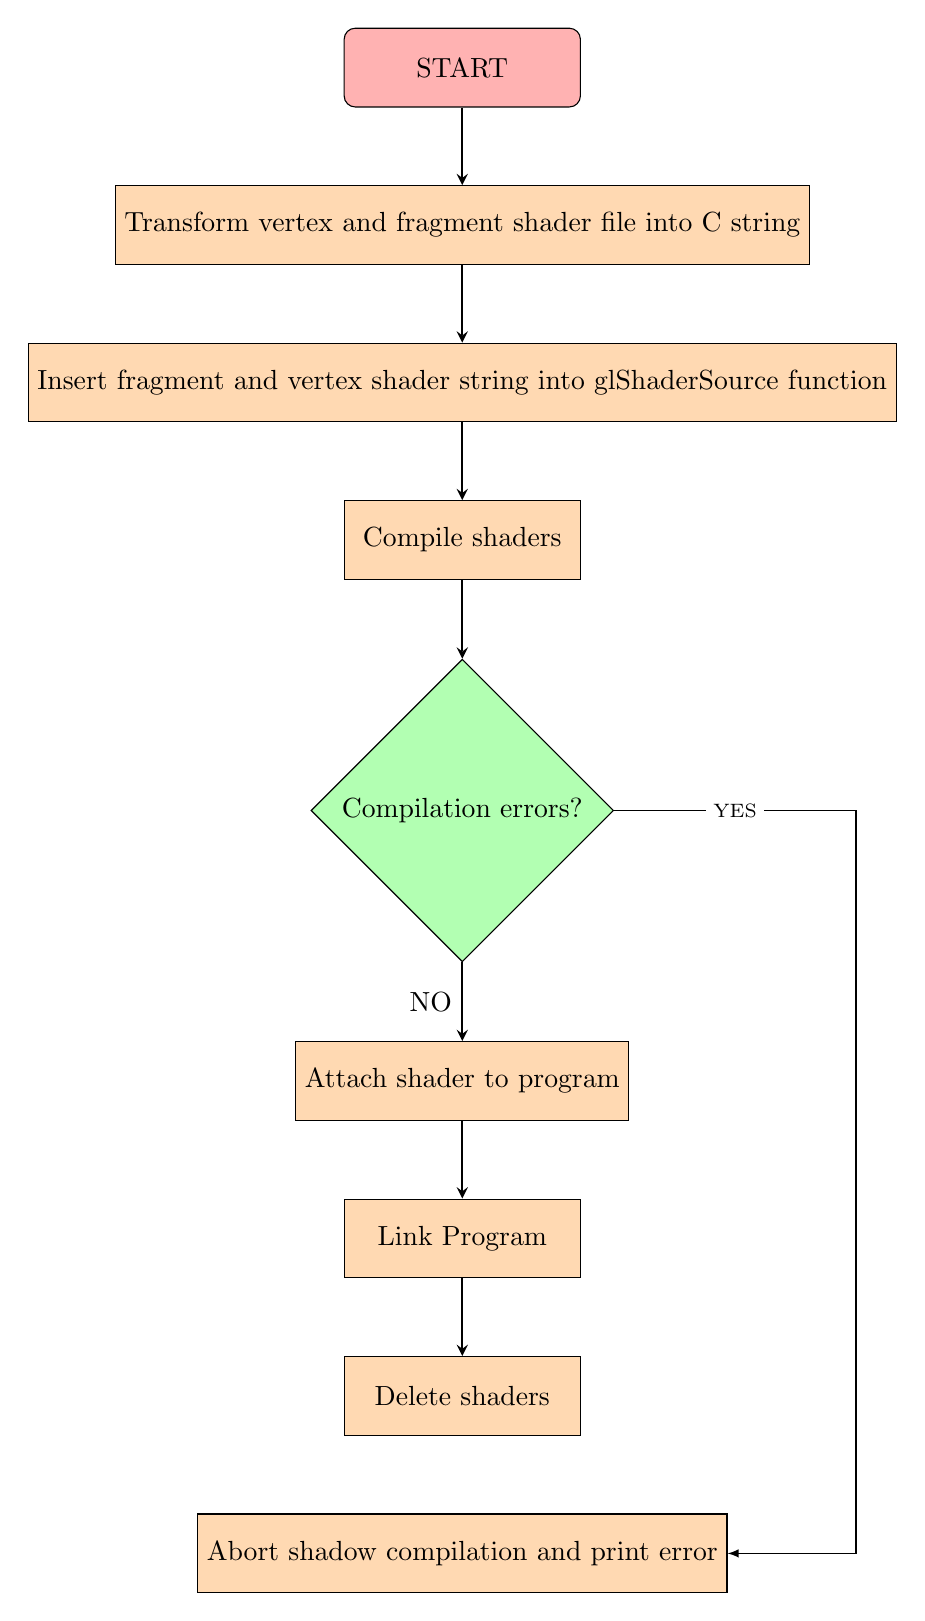
\begin{tikzpicture}[node distance=2cm]
		\node (beginMain) [startstop] {START};
		\node (setButtonClicked) [process, below of = beginMain]
			{Transform vertex and fragment shader file into C string};
	\node (buttonInterrupts) [process, below of = setButtonClicked] {Insert fragment and vertex shader string into glShaderSource function};
	\node (infiniteLoop) [process, below of = buttonInterrupts] {Compile shaders};
	\node (whichButton) [decision, below = 1 cm of infiniteLoop] {Compilation errors?};
	\node(idle) [process, below = 1 cm of whichButton] {Attach shader to program};
	\node(freeze) [process, below of = idle] {Link Program};
	\node (infiniteLoop2) [process, below of = freeze] {Delete shaders};
	\node (endCompass) [process, below of = infiniteLoop2] {Abort shadow compilation and print error};
	\draw [arrow] (beginMain) -- (setButtonClicked);
	\draw [arrow] (setButtonClicked) -- (buttonInterrupts);
	\draw [arrow] (buttonInterrupts) -- (infiniteLoop);
	\draw [arrow] (infiniteLoop) -- (whichButton);
	\draw [arrow] (whichButton) -- node [anchor=east] {NO} (idle);
	\draw [arrow] (idle) -- (freeze);
	\draw [arrow] (freeze) -- (infiniteLoop2);
	\draw [rectangle connector=5cm] (whichButton) to node[descr] {YES} (endCompass);
	\end{tikzpicture}
    \caption{Shader usage example}
\end{figure}

\begin{figure}[H]
    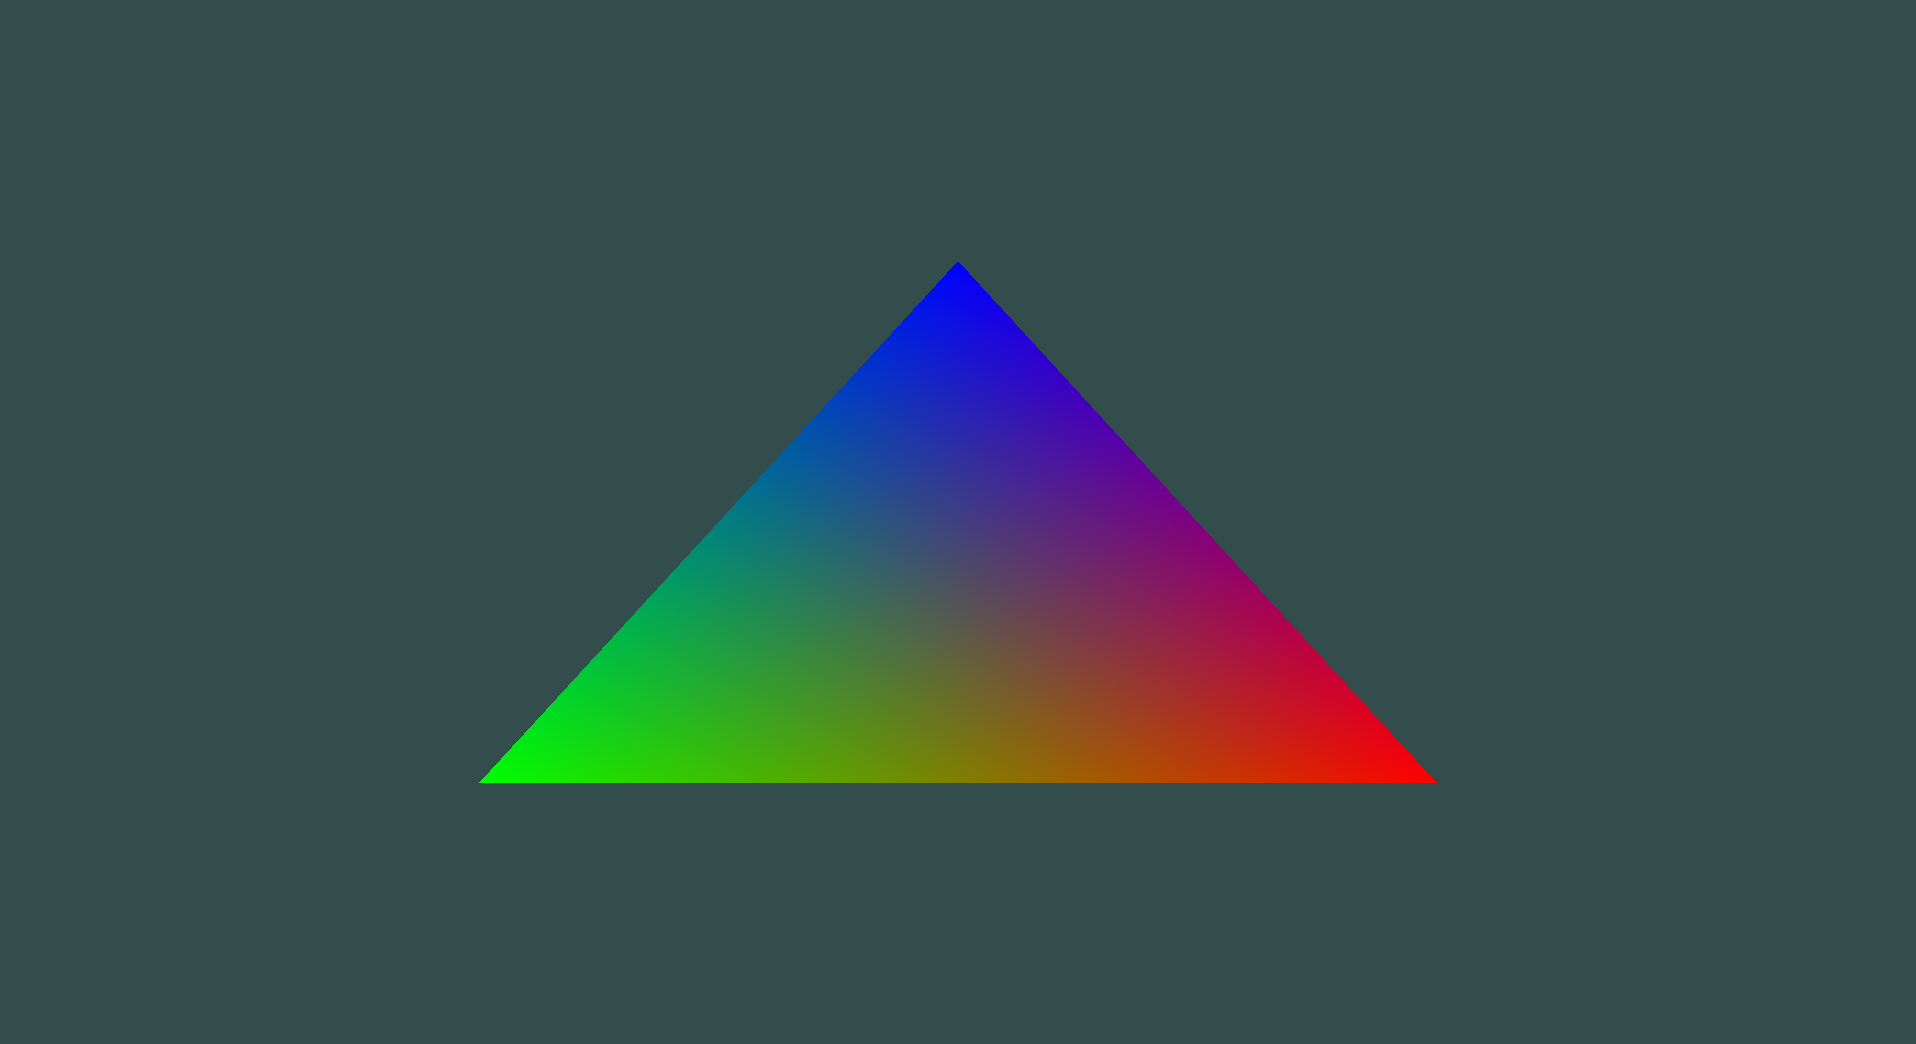
\includegraphics[width=\textwidth]{2}
    \centering
    \caption{More complex shader coloring the triangle based on the distance from the vertice}
\end{figure}

\section{Plans for future}
These are main areas I have to implement in future semester:
\subsection{Textures}
Used for drawing objects with custom, user imported pictures on them, crucial for making tiles have an unique look without need to manually add them using shaders and vertices. \\
More specifically:
\begin{itemize}
    \item Importing texture from a file to a program
    \item Wrapping texture around the object - For textures too small/big for an object  
    \item Filtering texture - Choosing which pixel should be colored on a texture 
    \item Combining textures with shaders - For coloring, adding effects to texture
\end{itemize}
\subsection{Transformation} 
Using OpenGL Mathematics library - GLM, objects in the game need to be able to move, both on them own and on player/user command. 
\subsection{User Interface}
Person using game engine needs to be able to:
\begin{itemize}
    \item Add, delete and modify shaders for given object (tiles, game background)
    \item Add, delete and replace textures for given object (tiles, game background)
    \item Test the game before building it
    \item Build the game itself 
\end{itemize}
Those elements need to be shown in the engine itself, using ImGui Menus

\section{Overview}
In total I feel confident in my ability to finish this project in next semester. \\ Having more time to spend on it, with the scope that I chose and good coding practices used so far which make my code reusable and modular I should be able to finish the thesis as planned.

\end{document}